% Options possibles
% init - pour le dossier d'initialisation
% francais ou english
% RandD - réservé aux PFE ayant le label R&D.
% Confidential - réservé aux PFE confidentiels
\documentclass[francais]{rapportPFE}  % pour une version française
%\documentclass[english]{rapportPFE}  % pour une version avec du texte en anglais

% L'option confidentiel a pour conséquence d'ajouter le filigrane "Confidentiel" sur la première et la dernière page
%  En fait, ce filigrane apparait sur toutes les pages numérotées 1 par Latex… 
% Pour le rajouter sur TOUTES les pages, décommenter la commande suivante
%\newwatermark[allpages,textalign=center,fontfamily=pbk,angle=55,scale=2.75,xpos=-1cm,ypos=1cm,color=lightgray]{Confidentiel}



\usepackage{listings}
\usepackage{fancyhdr}
\usepackage{caption} 
\usepackage{subfig}
% %%%%%%%%%%%%%%%%%%%%%%%%%%%%%%%%%%%%%%%%%%%
% titres du rapport
% %%%%%%%%%%%%%%%%%%%%%%%%%%%%%%%%%%%%%%%%%%%
% Version francaise
\titre{Développement d’interface graphique technologie web - faisabilité et évaluation}
% version anglaise
\title{Development of web-based graphical user interface - feasibility and evaluation}


% %%%%%%%%%%%%%%%%%%%%%%%%%%%%%%%%%%%%%%%%%%%
% Auteur du rapport
% %%%%%%%%%%%%%%%%%%%%%%%%%%%%%%%%%%%%%%%%%%%
\firstname{Colin}
%\middlename{Autre-Prénom}
\lastname{Thomas}



% %%%%%%%%%%%%%%%%%%%%%%%%%%%%%%%%%%%%%%%%%%%
% Informations sur le PFE
% %%%%%%%%%%%%%%%%%%%%%%%%%%%%%%%%%%%%%%%%%%%
% Information administratives
\dateDebutPFE{5 février 2024}
\dateFinPFE{26 juillet 2024}
\nomStructureAcceuil{Arturia}
\villeStructureAccuel{Grenoble}
\logoStructureAccueil{width=5.0cm}{graphics/LogoStructureAccueil} % si vous ne souhaitez pas mettre de logo pour la structure d'accueil, commentez cette ligne.
% paramètres de la commande logoStructureAccueil
% #1 = paramètre d'affichage du logo
% #2 = nom du fichier logo
% Pour plus de précision, cela correspond à la commande latex \includegrahics[#1]{#2}

% Encadrants.
% Penser à accorder la fonction avec le genre
\begin{encadrants}
% Fonction {Fonction}{ Prénom \Nom{Nom}}{Titre}{Structure}
  \referent{Référent}{Yann \Nom{Gripay}}{Maître de Conférences}{INSA Lyon}%
  \tuteur{Tuteur}{Timothée \Nom{Béhéty}}{Référent Technique Logiciels Compagnon}{Arturia (Grenoble)}
\end{encadrants}

% Date de la soutenance
\date{26 juin 2020}

% Réglage des entêtes et pieds de page
\fancyhf{}
\renewcommand{\headrulewidth}{0.2pt}
\renewcommand{\footrulewidth}{0.2pt}
\fancyhead[L]{\footnotesize{Un exemple d'en-têtes 
     et pieds de page}}
\fancyfoot[R]{\thepage}
\fancyfoot[C]{\footnotesize{---}}
\fancyfoot[L]{\footnotesize{\textit{Les 
     rédacteurs de la FAQ}}}


% %%%%%%%%%%%%%%%%%%%%%%%%%%%%%%%%%%%%%%%%%%%
% Rapport lui même
% %%%%%%%%%%%%%%%%%%%%%%%%%%%%%%%%%%%%%%%%%%%
\begin{document}
\maketitle


% ==========================================
% les résumés et les mots clés du rapport
% ==========================================

\begin{ResumeMotsCles}

% Version anglaise
% abstract no more than 12 lines.
\begin{resumeEn}
During my final internship, I had the opportunity to participate in the design and development of web interfaces for Arturia's next generation Companion Softwares. These softwares include the Arturia Software Center, Arturia's software store, and the Midi Control Center, Arturia's hardware configuration software. With the aim of updating aging software and experimenting with new graphic development technologies, my team decided to prototype a modular application bringing them together, utilizing web interfaces for the front-end.\\
My role involved developing web interfaces for the Arturia Software Center, integrating a C++ back-end developed by another team member. I also redesigned the Midi Control Center and prototyped the use of the Web MIDI API to communicate with Arturia devices on the web, as well as experimenting with the Web USB API to update device firmware.\\
Throughout my internship, I followed and participated in the conception of the modular application during weekly architecture meetings. \\
Working on such an innovative project at Arturia allowed me to explore innovative domains and deepen my teamwork and communication skills, which I had developed during my previous internships. 
\end{resumeEn}
% keywords
\keywords{Web~; Vue Nuxt~; Cross-Plateform~; Web APIs~; Modular App.}



% Version francaise
% Résumé pas plus de 12 lignes
\begin{resumeFr}
Durant mon stage de fin d'études, j'ai pu participer à la conception et au développement d'interfaces Web pour la nouvelle génération des Logiciels Compagnon d'Arturia. Ces logiciels sont l'Arturia Software Center, le magasin de logiciels d'Arturia, et le Midi Control Center, le logiciel de configuration de matériel Arturia. Dans l'optique de mettre à jour des logiciels vieillissant, et d'expérimenter de nouvelles technologies de développement graphique, mon équipe a décidé de prototyper une application modulaire les rassemblant, et d'utiliser des interfaces Web pour la partie front-end. \\% //TODO : modifier texte précédent
Mon rôle a été de développer des interfaces Web pour l'Arturia Software Center, en y intégrant un back-end C++ développé par un autre membre de l'équipe. J'ai également réalisé un nouveau design pour le Midi Control Center, et ai pu prototyper l'utilisation de l'API Web MIDI pour communiquer avec les appareils Arturia.  \\
J'ai pu par ailleurs, au long de mon stage, suivre et participer à la conception de l'application modulaire lors de réunions d'architecture hebdomadaires.\\
Travailler sur un projet aussi innovant à Arturia m'a permis d'expérimenter des domaines novateurs, mais aussi d'approfondir mes compétences de travail en équipe et de communication que j'ai pu développer lors de mes précédents stages. 
\end{resumeFr}

% Mots clés
\motscles{Web~; Vue Nuxt~; Cross-Plateforme~; Web APIs~; Application Modulaire.}
\end{ResumeMotsCles}


% ==========================================
% Remerciements éventuels
% ==========================================
% \begin{remerciements}
%   Merci à tous. Commenter cet environnement s'il n'est pas nécessaire.
% \end{remerciements}





% %%%%%%%%%%%%%%%%%%%%%%%%%%%%%%%%%%%%%%%%%%
% rapport proprement dit 
% %%%%%%%%%%%%%%%%%%%%%%%%%%%%%%%%%%%%%%%%%%

% ==========================================
% Sommaire (généré automatiquement)
% ==========================================
\setcounter{tocdepth}{3}
\tableofcontents
\cleardoublepage

% ==========================================
% Introduction
% ==========================================
%Contexte, 
%définition du problème, 
%aperçu des contributions, 
%plan du rapport



     
     
     
\section{Introduction.}

\subsection{Mise en contexte.}
J'ai réalisé mon stage de fin d'études chez Arturia, une société Grenobloise, fabricant d'instruments de musique numériques et électroniques, du 5 février au 26 juillet 2024. C'était l'entreprise que je souhaitais intégrer pour ce stage de fin d'études, non seulement car j'utilise et apprécie les produits et logiciels Arturia, mais aussi car je souhaitais me rapprocher du milieu de ma passion pour la musique. 
J'ai intégré pendant ce stage l'équipe Compagnon d'Arturia, qui m'a proposé un sujet de prototypage d'interfaces Web pour la nouvelle génération de deux de leurs logiciels, l'Arturia Software Center et le Midi Control Center. J'ai pu ainsi participer à la conception d'un logiciel modulaire rassemblant ces deux applications, développer des interfaces C++ préexistantes en Web, concevoir de nouvelles interfaces et prototyper l'utilisation d'APIs Web novatrices. Ce stage me permet de mettre en oeuvre les compétences de développement Web acquises pendant mon stage précédentj, ainsi que de mettre en pratique les connaissances théoriques que j'ai pu apprendre pendant mes études.
\subsection{Définition du problème.}

L'Arturia Software Center (ASC) et le Midi Control Center (MCC) sont deux logiciels vieillissants, qu'Arturia souhaite mettre à jour. Pour faire cela, l'entreprise souhaite mettre à l'épreuve de nouvelles technologies de développement graphique.

En effet, ces logiciels ont été développés respectivement en 2014 pour l'Arturia Software Center, et en 2013 pour le Midi Control Center. A ce moment, l'équipe Compagnon que j'intègre pour ce stage n'existait pas encore, et ces logiciels ont étés développés dans des technologies qui ne sont potentiellement pas optimales pour ces programmes.

Ainsi, l'équipe Compagnon a décidé de prototyper une application modulaire, nommée GeMAPS, qui rassemblerait l'Arturia Software Center et le Midi Control Center. Ce logiciel distribuerait et présenterait des pages Web pour ses interfaces utilisateur.

Le défi de mon équipe est donc de réussir à adapter un logiciel préexistant dans une nouvelle technologie, en en séparant le front-end et le back-end, et en réussissant à faire une application suffisemment modulaire pour qu'elle puisse intégrer à l'avenir de nouveaux éléments non encore définis.




\subsection{Aperçu des contributions.}
% //TODO : mettre à jour
Lors de ce stage, j'ai pu travailler sur plusieurs éléments : 
\begin{itemize}
    \setlength\itemsep{0em}
    \item Démontrer l'utilisation de multiples Frameworks Web (React, Angular, Vue, Vue Nuxt) dans une application modulaire C++ JUCE.
    \item Développer toutes les interfaces existantes C++ de l'Arturia Software Center en Vue Nuxt.
    \item Concevoir et développer les interfaces un Midi Control Center entièrement en Web, qui permet de configurer le clavier maître Arturia MiniLab3.
    \item Concevoir et développer l'interface du logiciel modulaire accueillant le Midi Control Center et l'Arturia Software Center.
    \item Prototyper l'implémentation de l'API Web MIDI pour communiquer avec les appareil Arturia en front-end Web uniquement.
    \item Expérimenter l'utilisation de l'API Web USB pour mettre à jour en Device Firmware Update les appareils Arturia, ainsi que de l'API FileSystem.
\end{itemize}
La majeure partie de mon travail était concentrée sur le développement des interfaces Web du Midi Control Center, ainsi que de l'Arturia Software Center, en étroite collaboration avec le membre de l'équipe travaillant sur le back-end. 

\subsection{Problématique et plan.}

La problématique de ce rapport de stage concerne d'une part, l'intégration d'interfaces Web dans un logiciel modulaire, et d'autre part, l'objectif de déplacement de l'intelligence logicielle du Midi Control Center dans le Web, impliquant l'expérimentation et la démonstration d'utilisation de l'API de diverses technologies Web novatrices.

% //TODO : plan


\section{Contexte.}

\subsection{Contexte du stage.}
% //TODO : ?????????? décider que mettre
\subsubsection{Intégration à l'équipe Compagnon}
Pour ce stage, j'ai été intégré à l'équipe Compagnon d'Arturia, une sous-équipe de l'équipe Système au sein du département R\&D. Sous la supervision de mon tuteur, Timothée Béhéty, qui dirige cette sous-équipe composée de 4 membres, j'ai collaboré étroitement avec Jean-Yves Tissot. Il est responsable du développement du back-end C++ de l'Arturia Software Center (ASC) et est le développeur du projet GeMAPS. Puisque l'équipe Compagnon se concentre exclusivement sur le développement en C++, j'ai sollicité l'expertise de Fabian Boilay, membre de l'équipe du site web d'Arturia, pour les revues de code.

\subsubsection{Méthodologie}

% méthodologie
% frontend ?


\subsection{Arturia.}

Arturia est un fabricant d'instruments de musique numériques et électroniques. La société est basée à Grenoble et développe des reproductions logicielles d'anciens synthétiseurs (analogiques et numériques), des claviers MIDI, des contrôleurs, des synthétiseurs analogiques et des interfaces audio. 

Il s'agit d'une entreprise employant 180 personnes, qui a été fondée en 1999. A sa création, ses deux fondateurs Frédéric Brun (actuel CEO d'Arturia) et Gilles Pommereuil ont commencé par créer des reproductions de synthétiseurs analogiques réputés au format virtuel, en commençant par développer l'Analog V, inspiré par les synthétiseurs Moog et en collaboration avec leur créateur. De nombreuses autres reproductions ont suivi, et sont devenues par la suite la V Collection, qui est la collection d'instruments virtuels d'Arturia, et la FX Collection, qui est son équivalent pour les effets audio.

Arturia a depuis élargi son catalogue à des instruments virtuels qui lui sont propres, plusieurs synthétiseurs analogiques renommés, différents contrôleurs MIDI ainsi que des cartes sons. 

L’équipe Compagnon dans laquelle je réalise mon stage s’occupe des logiciels accompagnants les produits Arturia, comme le gestionnaire de licences, le logiciel de configuration de matériel, ou encore des logiciels spécifique à chaque produits, comme par exemple l'application mobile qui accompagne le clavier AstroLab. 

\subsection{Présentation du sujet de stage.}


\subsubsection{Mission.}

L'Arturia Software Center (ASC) et le Midi Control Center (MCC) sont deux logiciels vieillissants, qu'Arturia souhaite mettre à jour. Pour faire cela, l'entreprise souhaite mettre à l'épreuve de nouvelles technologies de développement graphique.

En effet, ces logiciels ont été développés respectivement en 2014 pour l'Arturia Software Center, et en 2013 pour le Midi Control Center. A ce moment, l'équipe Compagnon que j'intègre pour ce stage n'existait pas encore, et ces logiciels ont donc étés développés par l'équipe Software, qui se spécialise dans le développement d'instruments virtuels. Ils ont opté pour l'utilisation de technologies de développement d'instruments virtuels, notamment le framework C++ JUCE, pour la création de ces outils. Cependant, une mise à jour de l'ASC et du MCC en utilisant des technologies différentes permettrait de se détacher des outils spécifiquement conçus pour les logiciels audio, potentiellement inadaptés à ces applications.

Ainsi, l'équipe Compagnon a décidé de prototyper une application modulaire qui rassemblerait l'Arturia Software Center et le Midi Control Center. Cette application serait capable de lancer des librairies C++ en tant que back-end, de servir en HTTP des pages Web statiques en tant que front-end, et d'afficher un host permettant de naviguer sur ces pages Web. De cette manière, l'Arturia Software Center et le Midi Control Center constitueraient = deux modules de cette application, chacun dotés d'un back-end sous forme de librairie C++, et d'un front end sous forme de page web statique, communiquant avec leur back-end par requêtes HTTP.\\

\subsubsection{Intérêt.}

Utiliser des interfaces web pour ces logiciels se révèle ainsi positif sur plusieurs points : 
\begin{itemize}
	\item Les technologies web sont plus efficaces pour créer rapidement des interfaces. En effet, les bibliothèques et outils pré-développés et libres d'accès sont nombreux, en constante évolution, et facile d'utilisation : on peut prendre pour exemple la fonctionnalité multilangue, qui est une fonctionnalité qui prend de l'importance pour Arturia, et qui demande beaucoup de ressources, pour un développement plus facile, classique et très documenté en technologies Web. De même, les framework Web offrent souvent une courbe d'apprentissage plus faible que le C++ ou autre langage qui n'est pas haut-niveau.
	\item Ceci permet, pour développer ces interfaces, de pouvoir rechercher des profils de développeurs front-end Web, ce qui est plus facile que de devoir rechercher des développeurs C++, puis de les former sur le framework JUCE, pour ensuite travailler sur des interfaces. En séparant le développement front-end du reste de l'application, ceci permet de rechercher des développeurs spécialisés dans leur domaines, et ainsi une meilleure évolutivité de l'équipe.
	\item Ensuite, cela permet de séparer le front-end du back-end. En effet, avoir une interface HTTP entre un back-end et un front-end permet de bien séparer ces deux parties. Ceci amène de la modularité et de la scalabilité, car chaque partie peut être modifiée sans affecter l'autre. On peut imaginer également une plus grande flexibilité technologique, car l'application Web pourrait être développée dans n'importe quel framework, sans impliquer de changement pour les librairies C++. Enfin, en isolant les accès directs au back-end, on peut ainsi mettre en place de meilleurs mesures de sécurité pour protéger les logiciels et les licences utilisateurs.
\end{itemize}

L'Arturia Software Center étant l'outil qui permet de gérer l'installation des logiciels, un back-end est forcément nécessaire pour soutenir le front-end. En effet, par design et pour des raisons de sécurités, les technologies Web n'ont pas accès au système de fichiers de l'utilisateur.

En revanche, la question se posera pour le Midi Control Center, dont la principale fonctionnalité est de communiquer par protocole Midi avec le contrôleur. Nous étudierons pendant ce stage la faisabilité d'un Midi Control Center entièrement réalisé en technologies Web.

\section{Etude bibliographique et analyse de l'existant.}
\subsection{L'Arturia Software Center existant.}

L’Arturia Software Center
\footnote{\url{https://www.arturia.com/support/asc-arturiasoftwarecenter}}
 (ASC) est le logiciel de gestion de licences et de
téléchargement de software d’Arturia : il est nécessaire pour tout utilisateur
souhaitant utiliser un logiciel Arturia. L'utilisateur peut naviguer parmi les logiciels disponibles sur l'Arturia Software Center sur la page "Explore Products", activer la licence du logiciel sur la page "My Products", le télécharger, le mettre à jour, gérer l'emplacement de ses fichiers dans les paramètres, ainsi que de rentrer le code d'un produit Arturia physique afin de bénéficier des logiciels qui l'accompagnent.

L’Arturia Software Center est composé de deux parties : 

Tout d'abord, une partie principale, qui est ce logiciel qui permet de gérer ses licences et ses téléchargements de logiciels Arturia, et fournit une interface graphique.

Ensuite, un logiciel nommé ASC Agent, qui fonctionne en arrière plan, et vérifie les licences utilisateur à chaque démarrage de produit Arturia, afin d'éviter toute fraude et téléchargement illégal.

\begin{center}
	\centering
	\includegraphics[width=0.6\textwidth]{graphics/asc_existant.png}
	\begin{tiny}
	\end{tiny}
	\captionof{figure}{Arturia Software Center (ASC) existant}
	\label{fig}
\end{center}

\subsection{Le Midi Control Center existant.}

Le Midi Control Center
\footnote{\url{https://support.arturia.com/hc/fr-fr/sections/4405740766098-MIDI-Control-Center}}
 (MCC) est le logiciel de configuration de matériel Arturia : il
permet de gérer les configurations et les paramètres des synthétiseurs et contrôleurs MIDI, ainsi que de faire les mises à jour firmware pour les synthétiseurs analogiques, cartes sons et claviers midis physiques d’Arturia. Il communique en norme MIDI avec les produits Arturia pour leur configuration.

Il est composé d'une page "Device Settings" permettant de modifier les paramètres généraux du contrôleur actuellement connecté (par exemple, son temps de mise en veille ou ses courbes de vélocité), une page "Controller Map" permettant de modifier les paramètres de chaque contrôle du contrôleur, (par exemple, modifier la note attribuée à une touche en particulier), et une page permettant d'importer ou d'exporter des templates de paramètres. Il est également possible d'effectuer une détection automatique de mises à jour disponibles pour le firmware du contrôleur.

\begin{center}
	\centering
	\includegraphics[width=0.6\textwidth]{graphics/mcc_existant.png}
	\begin{tiny}
	\end{tiny}
	\captionof{figure}{Midi Control Center (MCC) existant}
	\label{fig}
\end{center}


\subsection{L'API Web MIDI.}

L'API Web MIDI
\footnote{\url{https://developer.mozilla.org/en-US/docs/Web/API/Web_MIDI_API}}
fournit une manière pour les applications web d'interagir avec les périphériques MIDI connectés à l'ordinateur. Elle permet d'envoyer et de recevoir des messages MIDI, par exemple recevoir des messages de Note On / Note Off, mais aussi envoyer des messages Sysex permettant de modifier les paramètres du périphérique.

Actuellement, cette API n'est disponible que sur les navigateurs Safari et Chromium. Cependant, cela ne pose aucun problème pour notre application, car nous avons la liberté de choisir le navigateur. En l'occurence, celui que nous utilisons est celui de Juce, et il est basé sur Chromium pour Windows, et sur Safari pour Mac.

\subsection{Définitions nécessaires.}

Nous allons ici définir quelques termes propres au matériel de production musicale.
\paragraph{Synthétiseur analogique} \footnote{\url{https://fr.wikipedia.org/wiki/Synthétiseur_analogique}} 
:
 Un synthétiseur analogique est un synthétiseur qui utilise des circuits analogiques et des signaux électriques analogiques pour générer des sons par des techniques électroniques. Contrairement à un synthétiseur numérique, qui stocke et communique l'information en binaire, l'information sonore est transmise dans l'analogique en tant que variation de tension.
\paragraph{MIDI} \footnote{\url{https://fr.wikipedia.org/wiki/Musical_Instrument_Digital_Interface}} 
: Le Musical Instrument Digital Interface ou MIDI est un protocole de communication et un format de fichier dédiés à la musique, et utilisés pour la communication entre instruments électroniques, contrôleurs, séquenceurs, et logiciels de musique. Il s'agit du protocole standard du matériel électronique de musique. Il permet par exemple à un Contrôleur MIDI d'envoyer le signal qu'une certaine note a été pressée avec une certaine vélocité, permettant à un logiciel sur ordinateur de produire un son en conséquence. Dans le sens inverse, ce protocole permet à l'utilisateur de paramétrer son contrôleur MIDI en envoyant des signaux SYSEX, comportant les informations nécessaire sur le paramètre à modifier et la valeur à lui attribuer.
\paragraph{Contrôleur MIDI} \footnote{\url{https://troidecis.fr/musique/instrument-midi-definition}} 
:  Un contrôleur MIDI est un appareil utilisé pour envoyer des signaux MIDI à l'ordinateur où à un autre appareil (par exemple, un synthétiseur analogique). Il peut se présenter sous la forme d'un clavier de piano, de faders, de potentionmères, d'encodeurs, ou bien d'autres.
\paragraph{Synthétiseur virtuel :} Un synthétiseur analogique virtuel est un synthétiseur simulant le son de synthétiseurs analogiques par le biais de processeurs numérique. Il peut être utilisé sous la forme de Stand-Alone, c'est à dire sans logiciel qui l'entoure, en le contrôlant par exemple par un contrôleur MIDI, mais également et plus populairement sous la forme Plug-In, c'est à dire en tant que module à intégrer à un logiciel de Musique Assistée par Ordinateur.
\paragraph{Message Sysex}
\footnote{\url{https://steinberg.help/cubase_artist/v10.5/fr/cubase_nuendo/topics/midi_editors/midi_editors_sysex_messages_c.html}}
: Un message SysEx est un type de message MIDI permettant de régler les paramètres d'un périphérique MIDI, ce qui n'est pas adapté à la syntaxe normale du protocole MIDI.


\section{Propositions scientifiques et techniques.}
\subsection{Méthodologie de travail.}
\subsubsection{Organisation de l'équipe et réunions.}
L'équipe Compagnon dans laquelle j'ai travaillé se réunissait pour un stand-up chaque matin, où l'on disait ce qu'on a fait la veille, ce qu'on prevoyait de faire le jour-même. C'était aussi l'occasion de partager les problèmes rencontrés et de recueillir les avis de l'équipe.

Nous effectuions également une réunion d'architecture du projet GeMAPS tous les vendredi, où l'on concevait ensemble le projet sur lequel moi et Jean-Yves travaillions. 


\subsubsection{Git et revues de code.}
Pour mon projet, j'ai fonctionné avec Git. Travaillant seul, j'avais une branche principale, et une branche secondaire sur laquelle je faisais des modifications avant de faire une Merge Request (MR). Ainsi, je pouvais, pour des modifications importantes, demander la revue de Fabian Biolay sur mes modification avant de les intégrer à ma branche principale. J'ai eu ainsi 3 projets Git, que sont la page hôte qui accueille les deux applications, l'Arturia Software Center, et le Midi Control Center.

\subsection{Environnement technique.}

\subsubsection{Architecture modulaire.}
L'architecture modulaire que nous souhaitons développer se nomme GeMAPS, signifiant Generic Modular Architecture (With) Pluggable Services. 

Le choix de l'architecture modulaire se justifie ici sur plusieurs aspects : 
\begin{itemize}
    \item Un besoin de simplifier l'expérience utilisateur : en effet, les utilisateurs d'Arturia ont actuellement besoin de multiples logiciels Compagnon pour avoir un environnement Arturia fonctionnel, ce le qui rend donc plus difficile d'accès. L'équipe support a fait remonter de nombreuses plaintes d'utilisateurs ayant des difficultés à utiliser par exemple un clavier maître Arturia, et c'est donc une volonté de l'entreprise de simplifier l'expérience d'accueil utilisateur sur plusieurs projets. Par exemple, pour utiliser et mettre à jour le firmware d'un clavier maître Arturia, un utilisateur doit d'abord télécharger l'Arturia Software Center, s'en servir pour enregistrer le clavier, puis télécharger le Midi Control Center à l'aide de l'ASC, ce qui installe le driver par la même occasion, puis enfin télécharger la mise à jour sur le Midi Control Center.
    \item Le besoin de se tourner vers une architecture plus facilement évolutive, permettant une intéropérabilité entre les logiciels. En effet, nous pouvons remarquer des besoins communs entre les logiciels Arturia Software Center et Midi Control Center, ainsi que facilement imaginer vouloir réutiliser de nombreuses fonctionnalités pour de futurs modules.
\end{itemize}
C'est ainsi une approche qui répond aux besoins utilisateurs, tout en permettant des développements futurs plus efficaces.

\subsubsection{Architecture d'un module}

On pourra charactériser un module par aucune, une ou plusieurs pages Web, ainsi qu'aucune, une ou plusieurs librairies applicatives C++.

Par exemple, le Midi Control Center du Minilab3 est composé d'une seule page Web. Celle-ci se sert de l'API Web MIDI pour communiquer avec le clavier maître. Par le futur, pour permettre la mise à jour Firmware ou la sauvegarde de templates, une librairie C++ sera développée.

D'autre part, l'Arturia Software Center est composé de trois pages Web, que sont les trois onglets de l'Arturia Software Center actuel, ainsi que d'une librairie back-end C++, qui permet de mettre à disposition des end-points pour la connexion utilisateur, la récupération de produits, le téléchargement, et toute la partie en ligne ou applicative de l'ASC.

Cependant, plusieurs modules seront des cas spécifiques dans cette architecture modulaire :
\paragraph{Page Principale} : la page principale, qui permet de naviguer entre les modules, doit être celle qui est affichée de base, et ne doit pas être servie sur les mêmes endpoints que les autres pages.
\paragraph{Arturia Software Center} : Ce module a besoin d'une connexion : ainsi, nous n'afficherons qu'une page Web de connexion, au lieu des 3 onglets prévus, tant que l'utilisateur n'est pas connecté à son compte Arturia.



\subsubsection{Environnement technique de l'application GeMAPS.}

Si l'on retire les modules, l'application GeMAPS fonctionne en plusieurs parties, que l'on peut rassembler en deux groupes : le serveur, et l'hôte.

Le serveur crée une interface HTTP, qui permet de mettre à disposition des end-points pour tous les fichiers Web qu'affichera l'hôte, ainsi que tous les end-points back-end que les interfaces Web requêteront.

L'hôte affiche la page Web principale, et est nommé Unified Control Center (UCC). Nous utilisons pour l'instant le navigateur intégré au framework C++ Juce, qui intègre Internet Explorer (lui-même basé sur Chromium) sous Windows et WebKit sous Mac. Nous envisageons, pour le futur, d'utiliser Chromium Embedded Software (CEF), afin d'unifier les navigateurs sous tous les systèmes d'exploitation, et également afin d'avoir un contrôle plus grand sur le navigateur.


\begin{center}
	\centering
	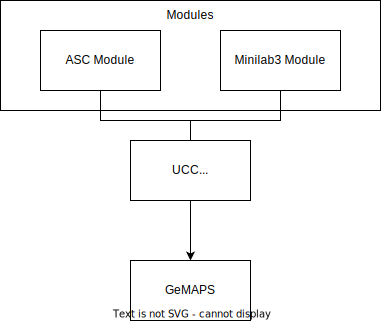
\includegraphics[width=0.5\textwidth]{graphics/gmaps.png}
	\begin{tiny}
	\end{tiny}
	\captionof{figure}{Architecture de l'application GeMAPS}
	\label{fig}
\end{center}

\subsubsection{Environnement technique frontend.}

Pour l'environnement technique frontend, j'ai pu prototyper dès le début du stage l'utilisation de différents frameworks Web dans l'application GeMAPS : React, Angular, et Vue.  

Pour développer les prototypes de l'Arturia Software Center et du Midi Control Center, le choix du framework m'a été laissé : je me sentais plus compétant sur Angular TypeScript, car c'était ce que j'avais utilisé durant le stage précédent. Ceci s'est révélé être une erreur, car cela ne correspondait pas à la stack technologique utilisée au sein de l'entreprise, notamment de l'équipe Web qui travaille avec Vue Nuxt. Afin de favoriser la cohérence de l'entreprise, ainsi que pour bénéficier des conseils d'experts dans le framework, il m'a été recommandé de refactoriser les projets en Vue Nuxt. Cette démarche a permis ainsi une meilleur uniformité dans l'entreprise, ainsi qu'une progression plus rapide de mes compétences personnelles. J'ai également adopté les autres charactéristiques d'environnement technique de l'équipe Web, que sont l'utilisation de Tailwind et du PostCSS pour les styles. 

Par ailleurs, j'utilise pour le Midi Control Center l'API Web MIDI, que l'on a pu définir plus tôt. 

\subsubsection{Environnement pour la gestion de projet}
L'équipe Compagnon utilise Trello pour la gestion de projet. L'équipe s'en sert pour gérer les tickets, distribuer les tâches, visualiser les tâches en attente de chaque projet ainsi que les tâches en cours.

\subsection{Propositions techniques / Implémentations}
\subsubsection{Prototypage d'utilisation de framework Web}
Mes premières tâches à Arturia fûrent de démontrer la possibilité d'utiliser différents frameworks Web dans l'application GeMAPS.
J'ai ainsi pu réaliser, en Vue, React et Angular, la reproduction d'un page de l'Arturia Software Center, ainsi que les afficher dans une page principale basique, permettant de naviguer entre les pages Web distribuées. 
Les résultats de ce prototypages sont que aucune différence n'est à observer entre ces différents frameworks, une fois l'application Web buildée : le point de différence majeur fut que l'architecture de fichiers buildés n'est pas la même par défault sur ces différentes technologies, et nécessite donc de lister les fichiers et répertoires à distribuer pour le serveur de fichiers de GeMAPS.



\begin{figure}%
    \centering
    \subfloat[\centering ]{{\includegraphics[width=6cm]{graphics/vue_demo.png} }}%
    \qquad
    \subfloat[\centering ]{{\includegraphics[width=6cm]{graphics/vue_demo2.png} }}%
    \caption{Page utilisée pour démontrer l'utilisation de différents frameworks dans GeMAPS}%
    \label{fig:example}%
\end{figure}


\subsubsection{Fonctionnalités clés de l'Arturia Software Center}
\paragraph{La connexion utilisateur}: La connexion utilisateur comporte ici plusieurs points de complexité. 

En effet, la connexion de l'Arturia Software Center déjà existant inclus la synchronisation, c'est à dire le moment où le backend vérifie que toutes les images et descriptions de produits sont prétéléchargées, récupère les dernières versions de logiciels mis à jour, et récupère les licenses actuellement possédées par l'utilisateur. Tout ceci se produit après que l'utilisateur ai entré un login et un mot de passe correct : on affiche alors une page de synchronization pour le faire attendre. S'est alors posée pour nous la question de l'implémentation dans une architecture où l'on a séparé le back-end et le front-end : comment prévenir le front-end que la synchronization s'est terminée ? Nous avons opté pour l'utilisation de Server-Sent Events (SSE). Ainsi, lorsque l'utilisateur se connecte, sa requête n'est pas répondue avant la fin de la synchronisation, auxquel moment il faudra le rediriger vers ses produits. En revanche, l'avancement de la synchronisation est partagée entre le back-end et le front-end par SSE envoyés par le back-end, prévenant soit du début, soit de la réussite, soit de l'échec de la synchronisation.
\begin{center}
    \centering
    \begin{minipage}{.5\textwidth}
    \centering
    \includegraphics[width=7cm]{graphics/disconnected.png}
    \captionof{figure}{Page de connexion de l'ASC}%
    \label{fig:test1}
    \end{minipage}%
    \begin{minipage}{.5\textwidth}
    \centering
    \includegraphics[width=7cm]{graphics/sync.png}
    \captionof{figure}{Page de synchronisation de l'ASC}%
    \label{fig:test2}
    \end{minipage}
    \end{center}

D'un autre côté s'est posée la question de l'auto-login, qui est une fonctionnalité implémentée par l'Arturia Software Center existant, et qui permet à l'utilisateur de n'avoir à se connecter qu'une fois sur sa machine. Dans notre cas, cela pose particulièrement problème, car nous démarrons le back-end et le front-end en même temps, et il faut donc au front-end savoir à quel étape de la connexion le back-end se trouve pour afficher les pages correspondantes. Nous avons décidé d'ajouter un end-point au back-end, qui permet, en cas d'auto-login, de demander si l'utilisateur est en cours de connexion, de synchronisation, ou si tout est déjà fini.

Enfin, le fait d'avoir 3 pages disponibles pour les 3 onglets de l'Arturia Software Center, même si ceux-ci sont déconnectés, était illogique d'un point de vue de l'expérience utilisateur : celui-ci voyait 3 fois la même page de connexion. Nous avons décidé de n'afficher qu'une page disponible de connexion sur la page principale de GeMAPS, tant que l'utilisateur n'est pas connecté. Ceci nécessite ainsi de partager le statut de connexion entre la page Web principale, et la page Web de l'Arturia Software Center. Nous avons décidé de passer par les cookies de navigateur pour partager cette information.

\begin{center}
    \centering
    \begin{minipage}{.5\textwidth}
    \centering
    \includegraphics[width=7cm]{graphics/disconnected.png}
    \label{fig:test1}
    \end{minipage}%
    \begin{minipage}{.5\textwidth}
    \centering
    \includegraphics[width=7cm]{graphics/connected.png}
    \label{fig:test2}
    \end{minipage}
    \captionof{figure}{Effet du statut de connexion sur la page principale de GeMAPS}%
    \end{center}

\paragraph{Installation de produits} ??????????????????????????
\paragraph{multilinguisme}: Le multilinguisme est une fonctionnalité essentielle pour d'Arturia, et qui est en cours de développement dans plusieurs projets. La facilité de développement multilingue, qu'amène la technologie Web est un autre avantage que montre mon prototype.

Pour développer cette fonctionnalité, j'ai utilisé les mêmes technologies que l'équipe Web d'Arturia, ce qui permet une uniformité et donc une meilleure efficacité lors du traitement des traductions. J'utilise ainsi le package @nuxtjs/i18n, et je crée une série de traductions pour chaque page et chaque composant Web.

Pour passer d'une langue à l'autre, j'ai créé un composant qui permet de choisir entre les langues disponibles.

\begin{center}
	\centering
	\includegraphics[width=0.5\textwidth]{graphics/languages.png}
	\begin{tiny}
	\end{tiny}
	\captionof{figure}{Composant de selection de langue}
	\label{fig}
\end{center}

\paragraph{Dark Mode}: Pareillement que le multilinguisme, le Dark Mode est une fonctionnalité commune et bien documentée en technologies Web. Pour le développer, j'ai utilisé l'attribut 'dark:' de Tailwind PostCSS pour créer un style sombre pour chaque page et composant WEB, et j'ai créé un composant permettant de sélectionner le mode voulu.

Pour développer cette fonctionnalité, j'ai utilisé les mêmes technologies que l'équipe Web d'Arturia, ce qui permet une uniformité et donc une meilleure efficacité lors du traitement des traductions. J'utilise ainsi le package @nuxtjs/i18n, et je crée une série de traductions pour chaque page et chaque composant Web.

Pour passer d'une langue à l'autre, j'ai créé un composant qui permet de choisir entre les langues disponibles.

\begin{center}
    \centering
    \begin{minipage}{.5\textwidth}
    \centering
    \includegraphics[width=7cm]{graphics/daymode.png}
    \label{fig:test1}
    \end{minipage}%
    \begin{minipage}{.5\textwidth}
    \centering
    \includegraphics[width=7cm]{graphics/darkmode.png}
    \label{fig:test2}
    \end{minipage}
    \captionof{figure}{Effet du Dark Mode sur l'ASC}%
    \end{center}


\paragraph{Favoris et Archivés}: Une des fonctionnalités qui m'ont été demandé pendant mon développement, a été de créer des catégories Favoris et Archivés pour les produits : en effet, en possédant de nombreux produits Arturia, la liste peut être longue, et il peut être fastidieux de naviguer longtemps pour chercher un produit qu'on utilise souvent.

J'ai ainsi ajouté une barre de boutons Favoris, Archivés et Tous sur l'Arturia Software Center, afin de pouvoir sélectionner quels produits afficher.
De même, j'ai ajouté des boutons Favoris et Archivés dans la page détails du produit. 
J'ai choisi de développer cette fonctionnalité de la manière la plus modulaire possible, afin qu'ajouter une catégorie supplémentaire à 'Favoris' ou 'Archivés' puisse être fait facilement.

\begin{center}
    \centering
    \begin{minipage}{.5\textwidth}
    \centering
    \includegraphics[height=4cm]{graphics/favorite.png}
    \label{fig:test1}
    \end{minipage}%
    \begin{minipage}{.5\textwidth}
    \centering
    \includegraphics[height=5cm]{graphics/favorite_details.png}
    \label{fig:test2}
    \end{minipage}
    \captionof{figure}{Fonctionnalité Favoris et Archivés}%
    \end{center}
% Image

\paragraph{Réactivité}: Une autre fonctionnalité très demandée, et facilitée par le Web, a été de faire un affichage dynamique, qui réagit au changement de taille de la fenêtre. En effet, l'Arturia Software Center déjà existant bloque sa taille, et ne peut pas être mis en plein écran.

Pour faire ceci, j'ai créé un affichage sous forme de cartes, afin que lorsque l'on agrandit la fenêtre en largeur, les produits qui deviennent trop larges sous forme de ligne, deviennent une grille de cartes de produits.

\begin{center}
    \centering
    \begin{minipage}{.5\textwidth}
    \centering
    \includegraphics[height=5cm]{graphics/small.png}
    \label{fig:test1}
    \end{minipage}%
    \begin{minipage}{.5\textwidth}
    \centering
    \includegraphics[height=5cm]{graphics/big.png}
    \label{fig:test2}
    \end{minipage}
    \captionof{figure}{Affichage des produits réagissant à la taille de la fenêtre.}%
    \end{center}



% Image

%\lstinputlisting[language=Python]{MonCode.py}
% \begin{lstlisting}[language=Python,caption={Programme inconnu},label=lst:Inconnu]
% import numpy as np
 
% def incmatrix(genl1,genl2):
%     m = len(genl1)
%     n = len(genl2)
%     M = None #to become the incidence matrix
%     VT = np.zeros((n*m,1), int)  #dummy variable
 
%     #compute the bitwise xor matrix
%     M1 = bitxormatrix(genl1)
%     M2 = np.triu(bitxormatrix(genl2),1) 
 
%     for i in range(m-1):
%         for j in range(i+1, m):
%             [r,c] = np.where(M2 == M1[i,j])
%             for k in range(len(r)):
%                 VT[(i)*n + r[k]] = 1;
%                 VT[(i)*n + c[k]] = 1;
%                 VT[(j)*n + r[k]] = 1;
%                 VT[(j)*n + c[k]] = 1;
 
%                 if M is None:
%                     M = np.copy(VT)
%                 else:
%                     M = np.concatenate((M, VT), 1)
 
%                 VT = np.zeros((n*m,1), int)
 
%     return M
% \end{lstlisting}



% Bibliographie
% Annexes éventuelles (en plus des 30 pages demandées)
\bibliographystyle{unsrt}
\bibliography{rapportPFE}
testtesttest


\appendix
\section{Acronymes.}
\paragraph{UCC}: Unified Control Center. C'est l'application hôte qui affiche le navigateur.
\paragraph{ASC}: Arturia Software Center. C'est l'application de gestion de logiciels Arturia.
\paragraph{MCC}: Midi Control Center. C'est l'application de gestion de controlleurs midi et synthétiseurs Arturia.

\section{Éléments majeurs de la conception.}

\section{Preuves de théorèmes.}
\end{document}
